\chapter{Deep Fractal based Hashing - DAsH}
 
 

\section{Consideraciones Iniciales}

\versal{S}e han propuesto   algoritmos de búsqueda  kNN aproximada basados en hashing para operaciones de búsqueda en conjuntos de datos de alta dimensionalidad debido a su alto desempeño  en  recuperación y bajo costo de almacenamiento. Estudios recientes, promueven el uso de la Red Neural Convolucional (CNN) con técnicas de hashing para mejorar la precisión de búsqueda. Sin embargo, existen retos a resolver para encontrar una solución práctica y eficiente para indexar las características de la CNN, tales como la necesidad de un intenso proceso de entrenamiento para lograr resultados precisos  y la dependencia crítica de los parámetros de datos. 


En \textit{Machine Learning} las imágenes se describen a menudo mediante las características visuales manuales.  Sin embargo, estas características manuales no pueden revelar el significado semántico de alto nivel (etiquetas o tags) de las imágenes, y a menudo limitan el rendimiento de la recuperación de imágenes \cite{Li:2015:RSS:2881665.2882186}. Así, para obtener esta información semántica tenemos que trabajar con la información de la etiqueta y procesar los datos en un modo supervisado. Inspirado por recientes avances en \acf{CNN} para problemas de clasificación de imágenes, detección de objetos, y muchas otras tareas de visión \cite{ImageNet,NIPS2013_5207,LiuWJJC12}, muchos métodos resolvieron el problema de la precisión de la recuperación de similitud utilizando CNN como extractor de características y luego construir un código hash compacto de preservación de similitud para la recuperación rápida de imágenes.   De nuevo, \textit{hashing} es ampliamente usado para recuperar imágenes a gran escala así como las búsquedas de video y documentos porque la representación compacta del código hash es esencial para el almacenamiento de datos y es razonable para las búsquedas de consultas \cite{conf/cvpr/ShenSLS15}.  Sin embargo, algunos inconvenientes basados en estos métodos de \textit{hashing} supervisados no se han resuelto completamente, como sigue:


\begin{itemize}

\item[-]  Existe un compromiso  entre error de clasificación y error de cuantificación: activaciones de capas inferiores son más generales \cite{DBLP:journals/corr/YosinskiCBL14}, así que el entrenamiento es más eficaz. Sin embargo, las capas inferiores tienen mapas de activaciones más grandes (muchos nodos), las cuales son más difíciles de codificar, lo que conduce a un compromiso. 
	
\item[-] Existe una dependencia de los valores de los parámetros para esquemas aproximados de búsqueda de similitud basados en hashing, que determinan el número de funciones hash y el número de tablas hash.  
 
\end{itemize}

En este trabajo  se propone una nueva técnica de \textit{hashing} supervisada,  llamada  \textit{Deep frActal based  Hashing} (DAsH),  diseñado para realizar una búsqueda de similitud aproximada escalable. Las contribuciones de nuestro trabajo son las siguientes. Primero,  introducimos y definimos un esquema jerárquico basado en CNN y optimizado usando la teoría fractal. Para superar la limitación de grandes activaciones en capas inferiores de CNN (salida de la última capa convolucional) reducimos su dimensionalidad usando autocodificadores a un sub-espacio óptimo. Luego indexamos esta nueva representación con un esquema de indexación LSH \cite{lshtutorial}.  Segundo, presentamos un nuevo método, basado en teoría fractal, que nos permite encontrar el número óptimo de funciones hash para un esquema aproximado de búsqueda de similitud basado en LSH.
  
 
\section{Deep Fractal based  Hashing - DAsH}

En esta sección, es propuesto \textit{Deep Fractal based  Hashing} (DAsH) diseñado para realizar una búsqueda aproximada escalable mediante un esquema de hash supervisado. Como se presentó en la sección 1, nuestra estrategia es usar la teoría de fractales para encontrar los óptimos sub-espacios para la última capa convolucional de salida de la red CNN, y el numero óptimo de funciones hash para una buena indexación. 

La figura \ref{fig:dash} ilustra la estructura del proceso de entrenamiento. La red consiste de tres tipos de capas: 1) Capas convolucionales con pesos pre-entrenados sobre Imagenet(\textit{transfer-learning}) y \textit{fine-tuning} en el conjunto de datos objetivo; 2) Una capa completamente conectada \textit{(full connected)} con la ultima capa \textit{softmax}; 3) Capa de \textit{autoencoders} los cuales son usados para reducir la dimensionalidad. \acf{CNN} está entrenado de extremo a extremo con etiquetas verdaderas. Utilizamos la salida de la última capa convolucional porque tiene la representación más general para el aprendizaje, pero tiene un inconveniente con una alta representación dimensional. Para superar el problema de alta dimensionalidad, reducimos al sub-espacio óptimo usando un autoencoder. Luego indexamos el subespacio óptimo obtenido por el autoencodificador con esquema LSH que, como hemos mencionado, también se sintoniza gracias a la teoría fractal. Al mismo tiempo, usamos otros n-autoencoders para aprender la representación de cada clase. Después, usaremos estos autocodificadores para mejorar el proceso de recuperación.  
\begin{figure}[htp]\centering
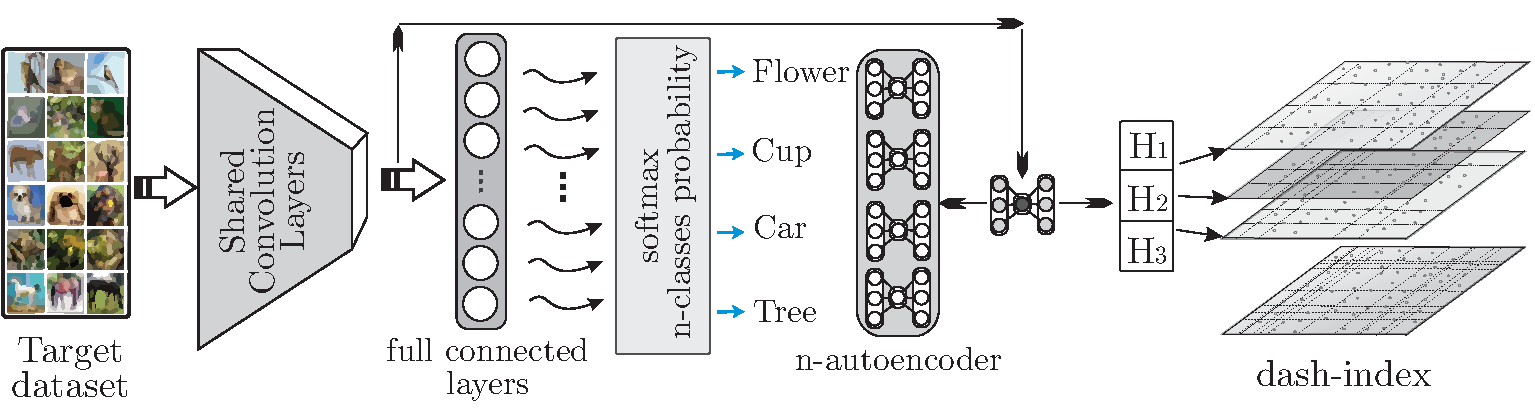
\includegraphics[width=1.0\columnwidth]{chapter6/DAsh_learning_final.pdf}
\caption{ DAsH. Proceso de entrenamiento e indexación. } 
\label{fig:dash}
\end{figure} 		

Como se mostró en \cite{citeulike:fractal:encoders} un algoritmo de reducción de dimensionalidad exitoso proyecta los datos en un espacio de características con dimensionalidad cercana a la dimensionalidad fractal (FD) de los datos en el espacio original y conserva las propiedades topológicas.  Por lo tanto, para encontrar la dimensionalidad objetivo ($m$) que necesitan las redes de autoencodificadores seguimos la siguiente heurística.  Empezamos con el valor $m_1 = 2^2$, calculamos la FD del nuevo espacio con sólo eso, luego incrementamos el valor en $m_2 = 2^3$, recalculamos la FD, y continuamos haciendo esto hasta algún $ t\ (m_t =  2^t)$ donde podemos ver una mejora en la dimensión fractal, lo que significa que más características no cambian la dimensionalidad fractal del conjunto de datos.
 
El segundo paso de nuestro procedimiento es la recuperación de la imagen vía  DAsH. Procesamos la imagen de consulta enviándola a través de CNN con el objetivo de obtener las clases $n$ más fuertes. En contraste con los algoritmos de aprendizaje de similitud existentes que aprenden la similitud de la característica de bajo nivel, nuestra similitud es la combinación de similitud semántica y nivel de hashing. Así que, la similitud de nivel semántico se calcula en primer lugar. Después de la comprobación de relevancia semántica, obtendremos las nuevas consultas ($q_1, q_2, ... q_n$) usando los  $n$ autoencoders más fuertes. La consulta es transformada en una nueva consulta de objetos ($q_1, q_2, ... q_n$) los cuales son escogidos para localizar los apropiados \textit{buckets}. Una vez que los \textit{buckets} son localizados, el conjunto de candidatos relevantes son formados.  Luego, los elementos del conjunto candidato se analizan exhaustivamente con el fin de recuperar sólo los objetos que satisfacen la condición de consulta. Este proceso es realizado para cada una de las  $L$ tablas hash . Este proceso es ilustrado en la Figura \ref{fig:qdash}.  
\begin{figure}[htp]
\centering
 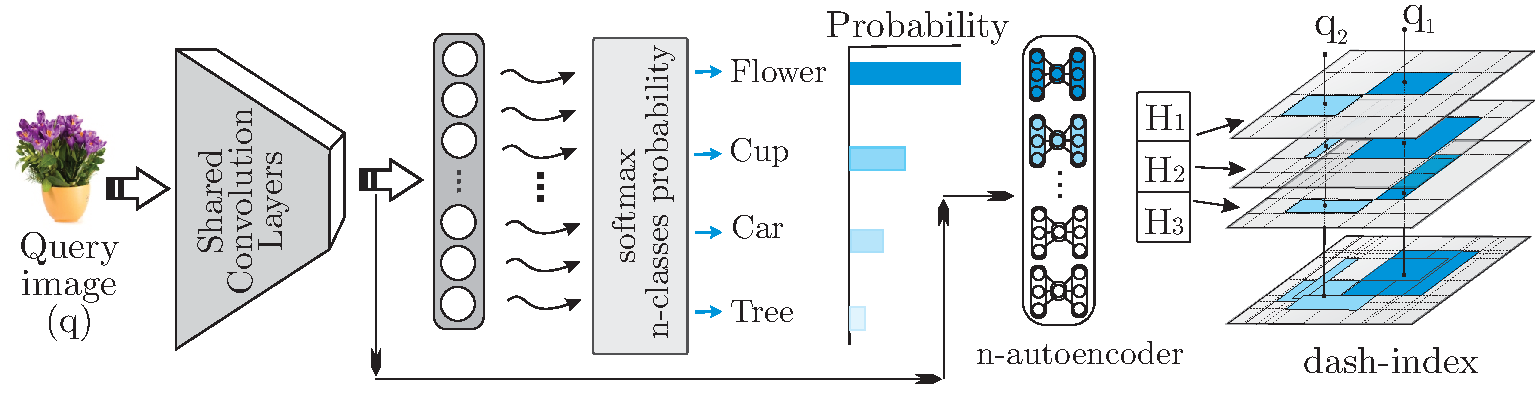
\includegraphics[width=1.00\columnwidth]{chapter6/DAsh_retrieval_final.pdf} 
 \caption{ DAsH. Proceso de recuperación. } 
\label{fig:qdash}
\end{figure} 
 
 \subsection{Usando Fractales para estimar los parámetros LSH}
 
Para afinar los parámetros LSH se utilizó una propiedad de la correlación de la dimensión fractal $\mathfrak{D}$, que puede describir estadísticamente un conjunto de datos. Además, la correlación de la dimensión fractal $\mathfrak{D}$ se puede estimar en tiempo lineal como se representa en \cite{traina2010fast}.

Estamos interesados en averiguar la escala de resolución $log(r)$ en la que hay aproximadamente $k$ objetos. Considerando la línea con pendiente $ \mathfrak{D} $ pasando en un punto definido como $<log (r), log(Pares (k))> $ la constante $ K_d $ usando la Ecuación \ref{eq:fractal} : 

%La idea de utilizar la Dimensión Fractal de Correlación para calcular los parámetros de LSH se aprovecha en una de las principales características de la Dimensión Fractal de Correlación $\mathfrak{D}$ que aseguran una distribución de la distancia entre los elementos del dataset original y una proyección óptima del sub-espacio se mantiene.  Además, la correlación dimensión fractal $\mathfrak{D}$ se puede estimar en tiempo lineal como se representa en \cite{Faloutsos:2000:SJS:335191.335412}  y \cite{traina2010fast}.  El exponente de distancia $\mathfrak{D}$ tal como está representado en \cite{Faloutsos:2000:SJS:335191.335412} es:

\begin{eqnarray}\label{eq:fractalk}
	   log(PC(r)) = \mathfrak{D} \times log (r) + K_p \nonumber\\
	   K_p   = log (Pairs (k)) - \mathfrak{D} \times log (r)
\end{eqnarray} 
	
Considerando otro punto $ <log(R), log(Pares(N))> $, la constante $ K_d $ se define como:
\begin{equation}\label{eq:fractalN}
    K_d    = log (Pairs(N)) - \mathfrak{D} \cdot log (R) 
\end{equation} 
Ahora, combinando Ecuaciones \ref{eq:fractalk}, \ref{eq:fractalN}, podemos definir el radio $r$ como:
\begin{equation}\label{eq:fractalR}
  r  =  R \cdot  exp (  \frac{log (Pairs (k)) - log (Pairs(N))}{ \mathfrak{D} } )    
\end{equation}
 
Usando la última ecuación \ref{eq:fractalR} descubrimos que el número óptimo de funciones hash $m$ para un índice basado en \textit{LSH} configurado para recuperar los $k$ vecinos más cercanos es proporcional al número de pares en una distancia $r$. Esto tiene sentido, porque un promedio de $k$ vecinos están dentro de una distancia dada $r$. Entonces, definimos:
\begin{equation}\label{eq:optimalM1}
   m \approx log (PC(r)) 
\end{equation}

combinando las ecuaciones \ref{eq:optimalM1} y \ref{eq:fractal} obtendremos que $m \approx \mathfrak{D} \cdot log (r)  $. Experimentalmente, confirmamos que el valor óptimo de $m$ es:

 \begin{equation}\label{eq:fractalm}
    m = (\left\lceil \mathfrak{D} + 1 \right\rceil  ) \cdot  log (r)
 \end{equation}

 
\section{Experimentos}

En esta sección, estamos interesados en responder a la siguiente pregunta: (a) ¿Qué tan preciso es nuestro modelo en la estimación de los parámetros LSH utilizando la dimensión fractal?; (B) ¿Cómo mejora nuestro método DAsH las otras implementaciones de LSH en términos de \textit{consultas de rendimiento} y \textit{precisión}?. El rendimiento del método DAsH se comparó con los de los dos métodos más conocidos, llamado Multi-probe LSH \cite{multiprobe} y LSH-Forest \cite{lshforest}. Todos los experimentos se realizaron en un workstation con Intel core i7  3.0Ghz (12 núcleos) CPU y 64Gb de RAM con cuatro tarjetas gráficas Geforce GTX 1080 GPU de 8Gb VRAM cada una.
 
Primero realizamos experimentos en ocho conjuntos de datos ampliamente utilizados usando características hechas a mano (AUDIO, CITIES, EIGENFACES, HISTOGRAMS, MGCOUNTY, RANDOMWALK, SYNTH16D, SYNTH6D, VIDEO) \footnote{\url{https://github.com/joselhuillca/fractal_dataset}} para evaluar nuestro método propuesto para estimar los parámetros LSH. Además de las características hechas a mano, también mostramos la eficacia de nuestros métodos cuando las características son extraídas por las Redes Neuronales Convolucionales profundas (CNN), realizamos este experimento en tres conjuntos de datos (MNIST\footnote{\url{http://yann.lecun.com/exdb/mnist/}}, CIFAR-10\footnote{\url{https://www.cs.toronto.edu/~kriz/cifar.html}}, SVHN\footnote{\url{http://ufldl.stanford.edu/housenumbers/}}) para evaluarlos en términos de \textbf{consultas de rendimiento} y \textbf{mean average precision (mAP)}. A continuación se describen los detalles de los experimentos y resultados.

\subsection{Experimento 1: Sintonización de parámetros LSH}

Los métodos basados en LSH reportan resultados eficientes cuando los valores $m$ (número de funciones hash) son elegidos.Para evaluar la eficacia del enfoque presentado para afinar los parámetros LSH utilizando la dimensión fractal, hemos trabajado en una variedad de datos sintéticos y reales. Tabla \ref{table:lshparams} resume las principales características y parámetros de los conjuntos de datos, incluyendo el número de elementos $N$, el número de atributos $d$, su dimensión intrínseca (fractal) $D$ y los parámetros LSH usando dos aproximaciones: el algoritmo de Andoni \footnote{\url{http://www.mit.edu/~andoni/LSH/}}  y nuestra propuesta basada en dimension fractal.  os resultados del experimento para el número de funciones de hash $m$ muestran que las estimaciones dadas por la ecuación \ref{eq:fractalm} son comparables con las obtenidas con el algoritmo E2LSH propuesto por Andoni utilizando hasta 10 veces menos tiempo.
 
\begin{table}[!t]
\caption{Optimal LSH Params using exhaustive e2lsh and the fractal based method.}
\label{table:lshparams}
\centering
\begin{footnotesize}
\begin{tabular}{c|r|r|r|r|r|r|r|r|r|r|}
    \cline{2-11}
    & \multicolumn{ 2}{|c|}{{\bf dataset}} & \multicolumn{ 3}{|c|}{{\bf fractal params}} & \multicolumn{ 2}{|c|}{{\bf e2lsh}} & \multicolumn{ 3}{|c|}{{\bf fractalsh}}  \\
    \cline{2-11}
    & \multicolumn{1}{c|}{$N$}    & \multicolumn{1}{c|}{$d$} & \multicolumn{1}{c|}{$\mathfrak{D}$}    & $log(R)$ & $log(CR)$   & $m$ & \multicolumn{1}{c|}{$time(s)$}    & \multicolumn{1}{c|}{$r$}  & $m$ & \multicolumn{1}{c|}{$time(s)$} \\
    \hline
\multicolumn{1}{|c|}{\bf audio}                 & 54387                 & 192      & 6.49     & -1.30      & 17.00       & \cellcolor[HTML]{f2f2f2}18                        & \cellcolor[HTML]{f2f2f2}64.20     & 0.14  & \cellcolor[HTML]{DFDFDF}16                    & \cellcolor[HTML]{DFDFDF}12.68                   \\
\multicolumn{1}{|c|}{\bf cities}                & 5507                  & 2        & 2.36     & 2.30       & 16.00       & \cellcolor[HTML]{f2f2f2}8                         & \cellcolor[HTML]{f2f2f2}16.45      & 4.16  & \cellcolor[HTML]{DFDFDF}6                     & \cellcolor[HTML]{DFDFDF}0.81                    \\
\multicolumn{1}{|c|}{\bf eigenfaces}            & 11900                 & 16       & 4.25     & -1.40      & 18.00       & \cellcolor[HTML]{f2f2f2}12                        & \cellcolor[HTML]{f2f2f2}42.28      & 0.13  & \cellcolor[HTML]{DFDFDF}13                    & \cellcolor[HTML]{DFDFDF}1.57                    \\
\multicolumn{1}{|c|}{\bf histograms}            & 4247                  & 256      & 2.50     & -0.81      & 16.01       & \cellcolor[HTML]{f2f2f2}6                         & \cellcolor[HTML]{f2f2f2}15.62      & 0.22  & \cellcolor[HTML]{DFDFDF}7                     & \cellcolor[HTML]{DFDFDF}6.12                    \\
\multicolumn{1}{|c|}{\bf mgcounty}              & 27282                 & 2        & 1.81     & 0.70       & 19.00       & \cellcolor[HTML]{f2f2f2}4                         & \cellcolor[HTML]{f2f2f2}87.96      & 0.27  & \cellcolor[HTML]{DFDFDF}4                     & \cellcolor[HTML]{DFDFDF}1.13                     \\
\multicolumn{1}{|c|}{\bf randomwalk}            & 10000                 & 1024     & 5.52     & 2.80       & 15.00       & \cellcolor[HTML]{f2f2f2}16                        & \cellcolor[HTML]{f2f2f2}50.60     & 10.16 & \cellcolor[HTML]{DFDFDF}17                    & \cellcolor[HTML]{DFDFDF}10.60                   \\
\multicolumn{1}{|c|}{\bf synth16d}              & 10000                 & 16       & 8.36     & -1.40      & 17.00       & \cellcolor[HTML]{f2f2f2}20                        & \cellcolor[HTML]{f2f2f2}27.20     & 0.18  & \cellcolor[HTML]{DFDFDF}18                    & \cellcolor[HTML]{DFDFDF}7.51                   \\
\multicolumn{1}{|c|}{\bf synth6d}               & 10000                 & 6        & 4.95     & -1.40      & 17.00       & \cellcolor[HTML]{f2f2f2}12                        & \cellcolor[HTML]{f2f2f2}28.16      & 0.14  & \cellcolor[HTML]{DFDFDF}12                    & \cellcolor[HTML]{DFDFDF}6.47                    \\
\multicolumn{1}{|c|}{\bf video}                 & 79094                 & 50       & 7.73     & -1.40      & 21.00       & \cellcolor[HTML]{f2f2f2}16                        & \cellcolor[HTML]{f2f2f2}1205.73     & 0.13  & \cellcolor[HTML]{DFDFDF}19                    & \cellcolor[HTML]{DFDFDF}92.54                   \\ 
\hline
\end{tabular}
\end{footnotesize}
\end{table}
%Gracias a esta relación entre los parámetros LSH y la dimensión fractal, podemos trabajar con datos a gran escala. Además, debido a la dimensión fractal se puede estimar en tiempo lineal podemos estimar óptimamente los parámetros de LSH en tiempo lineal también. 


\begin{table}[!htp]
\caption{Mean Average Precision(mAP), precision, and cumulative time spent to compute mAP for different methods on the MNIST, SVHN  and CIFAR-10 datasets. }
\label{table:map}
\centering
\begin{footnotesize}
\begin{tabular}{l|c|c|c|c|c|c|c|c|c|}
\cline{2-10}
                                           & \multicolumn{3}{c|}{\textbf{MNIST}}            & \multicolumn{3}{c|}{\textbf{SVHN}}             & \multicolumn{3}{c|}{\textbf{CIFAR-10}}         \\ \cline{2-10} 
                                           & \textbf{mAP} & \textbf{P (\%)} & \textbf{time(s)} & \textbf{mAP} & \textbf{P (\%)} & \textbf{time(s)} & \textbf{mAP} & \textbf{P (\%)} & \textbf{time(s)} \\ \hline
\multicolumn{1}{|l|}{\textbf{MpLSH  }}       & 0.86         & 0.95            & \cellcolor[HTML]{c8c8c8}19.58         & 0.71         & 0.73            & 8.09          & \cellcolor[HTML]{c8c8c8}0.83         & 0.89            & \cellcolor[HTML]{c8c8c8}122.45        \\ \hline
\multicolumn{1}{|l|}{\textbf{ITQ  }}         & 0.87         & 0.95            & 1297.32       & 0.70         & 0.80            & 8411.26       & 0.84         & 0.88            & 1056.83       \\ \hline
\multicolumn{1}{|l|}{\textbf{LOPQ  }}        & 0.86         & 0.90            & 119.21        & 0.71         & 0.74            & 613.65        & 0.83         & 0.88            & 528.20        \\ \hline
\multicolumn{1}{|l|}{\textbf{LSH-F  }}       & 0.85         & 0.96            & 217.33        & 0.61         & 0.78            & 365.90        & 0.86         & 0.89            & 365.47        \\ \hline
\multicolumn{1}{|l|}{\textbf{DAsH (Ours)}} & \cellcolor[HTML]{c8c8c8}0.93         & \cellcolor[HTML]{c8c8c8}0.98            & \cellcolor[HTML]{f2f2f2}20.82         & \cellcolor[HTML]{c8c8c8}0.74         & \cellcolor[HTML]{c8c8c8}0.84            & \cellcolor[HTML]{f2f2f2}10.34         & \cellcolor[HTML]{c8c8c8}0.88         & \cellcolor[HTML]{c8c8c8}0.91            & \cellcolor[HTML]{f2f2f2}125.37        \\ \hline
\end{tabular}
\end{footnotesize}
\end{table}
\subsection{Rendimiento de Recuperación} % OK
El objetivo de este experimento es medir el tiempo total dedicado a recuperar los objetos vecinos $k$-nearest. Las estructuras de datos que se compararon se probaron con valores específicos para las consultas. Por lo tanto, usamos $k = 1000$ cuando calculamos la métrica de Mean Average Precision ($mAP$) y $k = 25$ cuando calculamos la métrica de precisión $ (P(\%))$.

La Tabla  \ref{table:map} muestra la comparación en términos de mean average precision (mAP)  y tiempo de consulta para todos los métodos basados en hash. El método DAsH fue significativamente mejor que otros métodos; proporcionando hasta un mAP 10 \% mejor,  manteniendo un excelente tiempo de recuperación. Este resultado demuestra el potencial de impulsar las operaciones de consulta con el diseño de estructuras de índices especializados.
 
